\documentclass[a4paper]{article}

%\usepackage[utf8]{inputenc}

\usepackage{hyperref}
\usepackage{xcolor}
\usepackage{graphicx}
\usepackage[english]{babel}
\usepackage[T1]{fontenc}
\usepackage{url}
\usepackage{import}
\usepackage{multirow}
\usepackage{color}
\usepackage[numbered, framed]{matlab-prettifier}
\usepackage{fancyhdr}
\usepackage{amssymb}
\usepackage{tabu}
\usepackage{mathtools}
\usepackage[margin=2.5cm]{geometry}
\usepackage{listings}
\usepackage{titling}
\usepackage[utf8x]{inputenc}


\let\ph\mlplaceholder % shorter macro
\lstMakeShortInline"

\newcommand{\bnb}{\begin{nobreak}}
\newcommand{\enb}{\end{nobreak}}

\lstset{
  style              = Matlab-editor,
  basicstyle         = \mlttfamily,
  escapechar         = ",
  mlshowsectionrules = true,
}


\pretitle{%
  \begin{center}
  \LARGE
  
\includegraphics[width=\textwidth/4]{logo_unifi.png}\\[\bigskipamount]
}
\posttitle{\end{center}}
\date{}

\begin{document}



\title{\vspace{2cm}Elaborato di\\ \textbf{Calcolo Numerico}\\ Anno Accademico 2019/2020\vspace{3cm}}

\author{Niccolò \emph{Piazzesi} - \texttt{6335623} - \href{mailto:niccolo.piazzesi@stud.unifi.it}{\textit{niccolo.piazzesi@stud.unifi.it}}
   \and Pietro \emph{Bernabei} - \texttt{6291312} - \textit{pietro.bernabei@stud.unifi.it}}


\maketitle
\newpage
\tableofcontents


\newpage

\subsection{Esercizio 1} 
Sviluppando  in serie di Taylor in x si ottiene:\\
\[
f(x+h) = f(x) +  hf'(x) + \frac{h^2}{2}f''(x) + \frac{h^3}{6}f'''(x) + O(h^4)
\]
\[
f(x-h) = f(x) -  hf'(x) + \frac{h^2}{2}f''(x) - \frac{h^3}{6}f'''(x) + O(h^4)
\]
Sostituiamo i termini  nell'espressione iniziale:
\[
\frac{ f(x) -  hf'(x) + \frac{h^2}{2}f''(x) - \frac{h^3}{6}f'''(x) + O(h^4) -2f(x) + f(x) +  hf'(x) + \frac{h^2}{2}f''(x) + \frac{h^3}{6}f'''(x) + O(h^4)}{h^2} = \]

\[=\frac{h^2f''(x) + O(h^4)}{h^2} = f''(x) + O(h^2)
\]
\section{\textbf{Capitolo 2}}
\subsection{Esercizio 5}
Scrivere function Matlab distinte che implementino efficientemente i seguenti metodi
per la ricerca degli zeri di una funzione $f(x)$:
\begin{itemize}
    \item il metodo di Newton;
    \item il metodo delle secanti;
    \item il metodo di Steffensen:
\end{itemize}
\begin{eqnarray*}
    x_{n+1}=x_n - \frac{f(x_n)^2}{f(x_n + f(x_n)) - f(x_n)}, & & \mbox{n=0,1,...}
\end{eqnarray*}
Per tutti i metodi, utilizzare come criterio di arresto
\[
    \abs{x_{n+1} - x_n} \leq tol * (1 + \abs{x_n})
\]
essendo $tol$ una opportuna tolleranza specificata in ingresso. Curare particolarmente la robustezza
del codice.
\newline \textbf{Soluzione:} \newline
\begin{itemize}
    \item Metodo di Newton
          \lstinputlisting{capitolo2/es5_newton.m}
    \item Metodo delle secanti
          \lstinputlisting{capitolo2/es5_secanti.m}
    \item Metodo di Steffensen
          \lstinputlisting{capitolo2/es5_steffensen.m}
\end{itemize}

\subsection{Esercizio 6}
Utilizzare le $function$ del precedente esercizio per determinare una approssimazione
della radice della funzione
\[
        f(x) = x - cos(\frac{\pi}{2}x),
\]
per $tol = 10^{-3}, 10^{-6}, 10^{-9}, 10^{-12},$ partendo da $x_0 = 1$
(e $x_1 = 0.99$ per il metodo delle secanti). Tabulare i risultati,
in modo da confrontare le iterazioni richieste da ciascun metodo. Commentare
il relativo costo computazionale, in termini di valutazioni funzionali richieste.
\newline \textbf{Soluzione:}








Eseguendo lo script \nameref{cod:6}si ottengono i risultati contenuti nella tabella \ref{tab:6}
e nella figura \ref{fig:es6}. Come si può notare, il metodo di newton e il metodo delle secanti
convergono molto più rapidamente del metodo di bisezione e del metodo delle corde.
\begin{table}[h]
        \renewcommand\arraystretch{2}
        \begin{tabular}{|l l l l l|}
                \hline
                Metodo     & tolleranza$=10^{-3}$ & tolleranza$=10^{-6}$ & tolleranza$=10^{-9}$ & tolleranza$=10^{-12}$ \\
                \hline
                newton     & 5.94611646360541e-01 & 5.94611644056836e-01 & 5.94611644056836e-01 & 5.94611644056836e-01  \\
                secanti    & 5.94611646954077e-01 & 5.94611644056836e-01 & 5.94611644056836e-01 & 5.94611644056836e-01  \\
                steffensen & 5.94611681141925e-01 & 5.94611644056837e-01 & 5.94611644056836e-01 & 5.94611644056836e-01  \\
                \hline
        \end{tabular}
        \caption{valori approssimati con i metodi di Newton, secanti e Steffensen}
        \label{tab:6}
\end{table}
% \newpage
\begin{figure}[h!]
        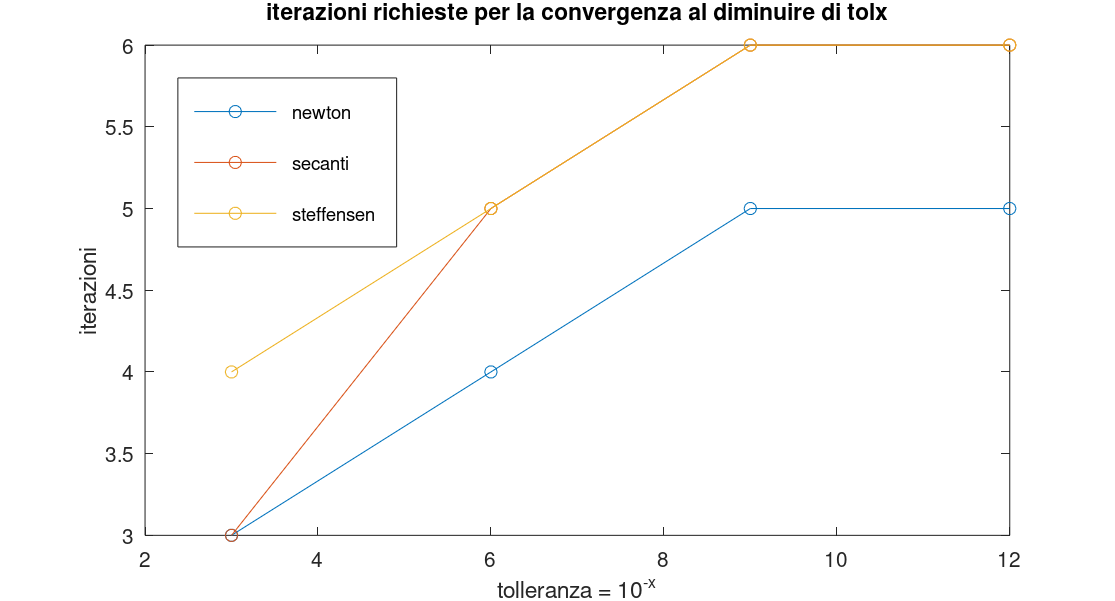
\includegraphics[scale=0.7]{capitolo2/es6_figure.png}
        \caption{iterazioni richieste}
        \label{fig:es6}
\end{figure}




\subsection{Esercizio 7}
Utilizzare le $function$ del precedente esercizio per determinare una approssimazione
della radice della funzione
\[
        f(x) = \left[x - cos(\frac{\pi}{2}x)\right]^3,
\]
per $tol = 10^{-3}, 10^{-6}, 10^{-9}, 10^{-12},$ partendo da $x_0 = 1$
(e $x_1 = 0.99$ per il metodo delle secanti). Tabulare i risultati,
in modo da confrontare le iterazioni richieste da ciascun metodo. Commentare
i risultati ottenuti.
\newline \textbf{Soluzione:}

Eseguendo lo script \nameref{cod:7} si ottengono i risultati contenuti nella tabella \ref{tab:7}
e nella figura \ref{fig:es7}. Come si può notare, il metodo di newton e il metodo delle secanti
convergono molto più rapidamente del metodo di bisezione e del metodo delle corde.
\begin{table}[ht]
        \centering
        \renewcommand\arraystretch{2}
        \resizebox{\columnwidth}{!}{
                \begin{tabular}{|l l l l l|}
                        \hline
                        Metodo                &        & newton                & secanti               & steffensen            \\
                        \hline
                        tolleranza$=10^{-3}$  & \vline & 5.969479343078770e-01 & 5.991437227787725e-01 & 5.973965526716639e-01 \\
                        tolleranza$=10^{-6}$  & \vline & 5.946140179818806e-01 & 5.946156634766230e-01 & 5.946143706333854e-01 \\
                        tolleranza$=10^{-9}$  & \vline & 5.946116464662755e-01 & 5.946116487688006e-01 & 5.946130329177074e-01 \\
                        tolleranza$=10^{-12}$ & \vline & 5.946116440592810e-01 & 5.946116440610053e-01 & 5.946130329177074e-01 \\
                        \hline
                \end{tabular}
        }
        \caption{Valori approssimati per $x - cos^{3}$ con i metodi di Newton, secanti e Steffensen}
        \label{tab:7}
\end{table}
\begin{figure}[!ht]
        \centering
        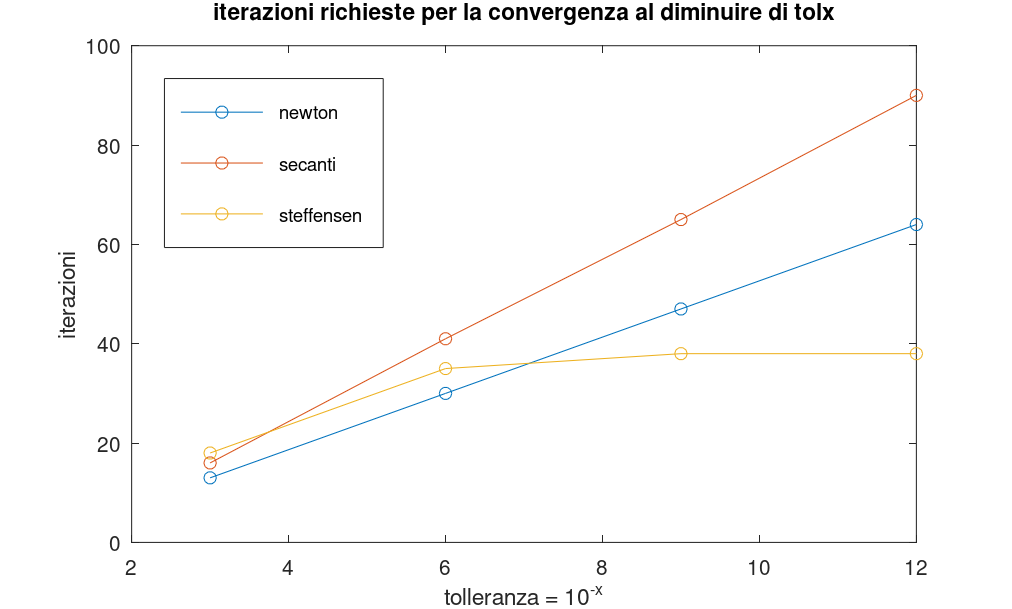
\includegraphics[width=16cm,height=12cm,keepaspectratio]{capitolo2/es7_figure.png}
        \caption{Valori approssimati per $x - cos^{3}$ con i metodi di Newton, secanti e Steffensen}
        \label{fig:es7}
\end{figure}
\FloatBarrier
In iterazione $38$ la funzione con metodo di Steffensen falliscie con valori di tolleranza
$10^-9$ e $10^-12$. Ed infatti, si vede che in questi valori la figura \ref{fig:es7}
rimane costante rispetto iterazioni. Questo fallimento dato da divizione a zero.
\newline \textbf{Costo computazionale} \newline
È possibile valutare i costi computazionali dei algoritmi verificando il numero
di funzioni richiamate all'interno dei codici, mediante feval:
\begin{itemize}
        \item Newton: $2i$, $i=1:maxit$;
        \item Secanti: $1 + i$, $i=1:maxit$;
        \item Steffensen: $2i$, $i=1:maxit$;
\end{itemize}


\section{\textbf{Capitolo 3}}
\subsection{Esercizio 8}
Scrivere una function Matlab,
\begin{lstlisting}[language=Matlab]
    function x = mialu(A, b)
\end{lstlisting}
che, data in ingresso una matrice $A$ ed un vettore $b$, calcoli la soluzione
del sistema lineare $Ax = b$ con il metodo di fattorizzazione $LU$ con pivoting parziale.
Curare particolarmente la scrittura e l'efficienza della function,
e validarla su due esempi non banali, generati casualmente,
di cui sia nota la soluzione.
\newline \textbf{Soluzione:}
\lstinputlisting[language=Matlab]{capitolo3/es8_lu.m}
\subsection{Esercizio 9}
Scrivere una function Matlab,
\begin{lstlisting}
function x = mialdl(A, b)
\end{lstlisting}
che, dati in ingresso una matrice sdp $A$ ed un vettore $b$, calcoli la soluzione
del corrispondente sistema lineare utilizzando la fattorizzazione $LDL^T$.
Curare particolarmente la scrittura e l'efficienza della function,
e validarla su due esempi non banali, generati casualmente, di cui sia nota la soluzione.
\newline \textbf{Soluzione:}

\lstinputlisting{matlab/capitolo3/mialdl.m}
Eseguendo lo script \nameref{cod:9} si ottengono i risultati contenuti nelle
tabelle \ref{tab:9_1} e \ref{tab:9_2}.

Prima sistema lineare è
\[
   \begin{bmatrix}
      166 & 105 & 161 & 132 \\
      105 & 119 & 151 & 98  \\
      161 & 151 & 239 & 144 \\
      132 & 98  & 144 & 131
   \end{bmatrix}
   \begin{bmatrix}
      x_{1} \\
      x_{2} \\
      x_{3} \\
      x_{4}
   \end{bmatrix}
   =
   \begin{bmatrix}
      5  \\
      10 \\
      6  \\
      2
   \end{bmatrix}
\]
Invece seconda sistema lineare è
\[
   \begin{bmatrix}
      45 & 27 \\
      27 & 18
   \end{bmatrix}
   \begin{bmatrix}
      x_{1} \\
      x_{2}
   \end{bmatrix}
   =
   \begin{bmatrix}
      2 \\
      5
   \end{bmatrix}
\]
Eseguendo la funzione creata \lstinline{mialdl} e comando interno di
matlab \lstinline{A\b}, possiamo confrontare il risultati di funzione
scritta con quello realizzato nativamente in matlab.
\begin{table}[ht]
   \centering
   \renewcommand\arraystretch{2}
   \begin{tabular}{|l | c c |}
      \hline
      $x$     & $mialdl$               & $A \backslash b$       \\
      \hline
      $x_{1}$ & 9.752409097697867e-02  & 9.752409097697871e-02  \\
      $x_{2}$ & 2.974225536634357e-01  & 2.974225536634358e-01  \\
      $x_{3}$ & -1.315833858151011e-01 & -1.315833858151011e-01 \\
      $x_{4}$ & -1.608594100046056e-01 & -1.608594100046056e-01 \\
      \hline
   \end{tabular}
   \caption{Confronto di soluzioni di \lstinline{mialdl} e $A \backslash b$ per primo sistema}
   \label{tab:9_1}
\end{table}
\begin{table}[ht]
   \centering
   \renewcommand\arraystretch{2}
   \begin{tabular}{| l | c c |}
      \hline
      $x$     & $mialdl$               & $A \backslash b$       \\
      \hline
      $x_{1}$ & -1.222222222222222e+00 & -1.222222222222221e+00 \\
      $x_{2}$ & 2.111111111111110e+00  & 2.111111111111110e+00  \\
      \hline
   \end{tabular}
   \caption{Confronto di soluzioni di \lstinline{mialdl} e $A \backslash b$ per secondo sistema}
   \label{tab:9_2}
\end{table}
\FloatBarrier

\subsection{Esercizio 10}
Data la function Matlab
\lstinputlisting{capitolo3/es10_linsis.m}
che crea sistemi lineari casuali con soluzione nota, risolvere, utilizzando la \textit{function} \lstinline{mialu}, i sistemi
lineari generati da \lstinline{[A,b]=linsis(10,1)} e \lstinline{[A,b]=linsis(10,10)}. Commentare l'accuratezza dei
risultati ottenuti, dandone spiegazione esaustiva.
\newline \textbf{Soluzione:} \newline
\begin{lstlisting}
>> [A, b] = linsis(10, 1); es8_lu(A,b)
ans =

    1
    2
    3
    4
    5
    6
    7
    8
    9
   10

>> [A, b] = linsis(10, 10); es8_lu(A,b)
ans =

  -307.6448
   386.6526
   184.3573
  -342.4373
   185.5085
   551.9206
  -137.7750
    70.6324
    -4.2105
  -608.0000

>>
\end{lstlisting}
Nel \textbf{primo caso} notiamo che l'errore é uguale a zero, infatti abbiamo che i soluzioni di $A$
sono tutti come aspettati: \lstinline{ans = [1; 2; 3; 4; 5; 6; 7; 8; 9; 10]}
\newline
Considerando che la soluzione con perturbazioni consiste nel risolvere il sistema
lineare $A(\epsilon)x(\epsilon) = b(\epsilon)$, dato che $\epsilon = 0 \rightarrow x(0) = x$
la soluzione senza perturbazione.
\newline
\newline
Nel \textbf{secondo caso} calcolando il numero di condizionamento
$K(A^T\cdot A) = \|A^T A\|\cdot\|(A^T A)^{-1}\|$ abbiamo che $K = 10^{16}$
Avendo $k \gg 1$ si ha un mal condizionamento del problema.

\subsection{Esercizio 11}
Scrivere una function Matlab,
\begin{lstlisting}[language=Matlab]
    function [x,nr] = miaqr(A, b)
\end{lstlisting}
che, data in ingresso la matrice $A$ $m \times n$, con $m \geq n = rank(A)$, ed un vettore $b$ di lunghezza
$m$, calcoli la soluzione del sistema lineare $Ax = b$ nel senso dei minimi quadrati e, inoltre, la
norma, $nr$, del corrispondente vettore residuo. Curare particolarmente la scrittura e l'efficienza della
\textit{function}. Validare la \textit{function} $miaqr$ su due esempi non banali, generati casualmente, confrontando
la soluzione ottenuta con quella calcolata con l'operatore Matlab.
\newline \textbf{Soluzione:}
\lstinputlisting[language=Matlab]{capitolo3/es11_qr.m}
\subsection{Esercizio 12}
Scrivere una function Matlab,
\begin{lstlisting}
function [x,nr] = miaqr(A, b)
\end{lstlisting}
che, data in ingresso la matrice $A$ $m \times n$, con $m \geq n = rank(A)$, ed un vettore $b$ di lunghezza
$m$, calcoli la soluzione del sistema lineare $Ax = b$ nel senso dei minimi quadrati e, inoltre, la
norma, $nr$, del corrispondente vettore residuo. Curare particolarmente la scrittura e l'efficienza della
\textit{function}. Validare la \textit{function} \lstinline{miaqr} su due esempi non banali,
generati casualmente, confrontando la soluzione ottenuta con quella calcolata con l'operatore Matlab.
\newline \textbf{Soluzione:}

\lstinputlisting{matlab/capitolo3/miaqr.m}
Eseguendo lo script \nameref{cod:12} si ottengono i risultati contenuti nelle
tabelle \ref{tab:12_1} e \ref{tab:12_2}.

Prima sistema lineare è
\[
   \begin{bmatrix}
      3  & 9 & 8 & 9 \\
      4  & 1 & 9 & 1 \\
      10 & 2 & 6 & 1 \\
      9  & 3 & 8 & 9
   \end{bmatrix}
   \begin{bmatrix}
      x_{1} \\
      x_{2} \\
      x_{3} \\
      x_{4}
   \end{bmatrix}
   =
   \begin{bmatrix}
      3 \\
      1 \\
      1 \\
      9
   \end{bmatrix}
\]
Invece seconda sistema lineare è
\[
   \begin{bmatrix}
      6  & 6 \\
      10 & 7 \\
      6  & 9
   \end{bmatrix}
   \begin{bmatrix}
      x_{1} \\
      x_{2}
   \end{bmatrix}
   =
   \begin{bmatrix}
      10 \\
      8  \\
      10
   \end{bmatrix}
\]
Eseguendo la funzione creata \lstinline{miaqr} e comando interno di
matlab \lstinline{r\c}, possiamo confrontare il risultati di funzione
scritta con quello realizzato nativamente in matlab.
\begin{table}[ht]
   \centering
   \renewcommand\arraystretch{2}
   \begin{tabular}{|l | c c |}
      \hline
      $x$     & $miaqr$                & $r \backslash c$       \\
      \hline
      $x_{1}$ & 1.491803278688525e-01  & 1.491803278688524e-01  \\
      $x_{2}$ & -8.508196721311473e-01 & -8.508196721311487e-01 \\
      $x_{3}$ & 1.475409836065585e-02  & 1.475409836065600e-02  \\
      $x_{4}$ & 1.121311475409836e+00  & 1.121311475409836e+00  \\
      \hline
   \end{tabular}
   \caption{Confronto di soluzioni di \lstinline{miaqr} e $r \backslash c$ per primo sistema}
   \label{tab:12_1}
\end{table}
\FloatBarrier
\begin{table}[ht]
   \centering
   \renewcommand\arraystretch{2}
   \begin{tabular}{| l | c c |}
      \hline
      $x$     & $miaqr$               & $r \backslash c$      \\
      \hline
      $x_{1}$ & 8.130081300812995e-02 & 8.130081300813012e-02 \\
      $x_{2}$ & 1.162601626016260e+00 & 1.162601626016260e+00 \\
      \hline
   \end{tabular}
   \caption{Confronto di soluzioni di \lstinline{miaqr} e $r \backslash c$ per secondo sistema}
   \label{tab:12_2}
\end{table}
Per dimostrare che risultato è corretto stato utilizzato il metodo discritto sul
\href{https://it.mathworks.com/help/matlab/ref/qr.html}{pagina di descrizione di funzione qr}
\FloatBarrier

\subsection{Esercizio 13}
Utilizzare la \textit{function} $miaqr$ per risolvere, nel senso dei minimi quadrati,
i sistemi lineari sovradeterminati
\begin{eqnarray*}
    \mbox{A x = b,} & & \mbox{(D*A)x = (D*b)}
\end{eqnarray*}
definiti dai seguenti dati:
\begin{lstlisting}
A = [ 1 3 2; 3 5 4; 5 7 6; 3 6 4; 1 4 2 ];
b = [ 15 28 41 33 22 ]';
D = diag(1:5);
\end{lstlisting}
Commentare i risultati ottenuti.
\newline \textbf{Soluzione:}

\lstinputlisting{./capitolo3/es13.m}
Il risultato finale è $ ris =\left(\begin{array}{c}
    1 \\
    2 \\
    3 \\
\end{array}\right)$  

\subsection{Esercizio 14}

\begin{table}[h]
\begin{tabular}{|l l|}
        \hline
        A$\backslash$b & (A’*A)$\backslash$(A’*b)\\
        \hline
        1.0000& 3.5759 \\
    	2.0000&-3.4624   \\
    	3.0000&  9.5151\\
    	4.0000&-1.2974\\
    	5.0000& 7.9574\\
    	6.0000& 4.9125\\
    	7.0000& 7.2378\\
    	8.0000& 7.9765\\
        \hline
\end{tabular}
\caption{valori approssimati}
\label{tab:14}     
\end{table}

L'espressione $A \backslash b$ risolve in matlab,  il sistema di equazioni lineari nella forma matriciale $A\cdot x=b$ per x.
L'espressione $(A^{T}\cdot A) \backslash (A^{T} \cdot b)$, è matematicamente la stessa operazione dell'espressione precedente, solamente che si moltiplica le due componenti per la trasposta di A. 
La matrice A viene calcolata usando la funzione vander() che genera una matrice di tipo Vandermonde, la quale è  mal condizionata. Usando la funzione cond() sulla matrice A si ottiene una condizionamento pari a: 1.5428e+09.Nella prima espressione, questo malcondizionamento non influisce sul risultato.Invece nella seconda espressione eseguendo la prima parentesi tonda, il condizionamento è pari a: 4.4897e+18. Questo fa si che eseguendo la divisione tra una matrice mal condizionata e il vettore, il risultato presenta degli errori.


\newpage
\section{\textbf{Capitolo 4}}


\newpage
\section{\textbf{Capitoli 5/6}}

\newpage
\pagenumbering{roman}


\end{document}
